\thispagestyle{doithoaitoanhocnone}
\pagestyle{doithoaitoanhoc}
\everymath{\color{doithoaitoanhoc}}
\graphicspath{{../doithoaitoanhoc/pic/}}
%\blfootnote{$^1$\color{doithoaitoanhoc}Viện Toán học Việt Nam.}
\begingroup
\AddToShipoutPicture*{\put(0,616){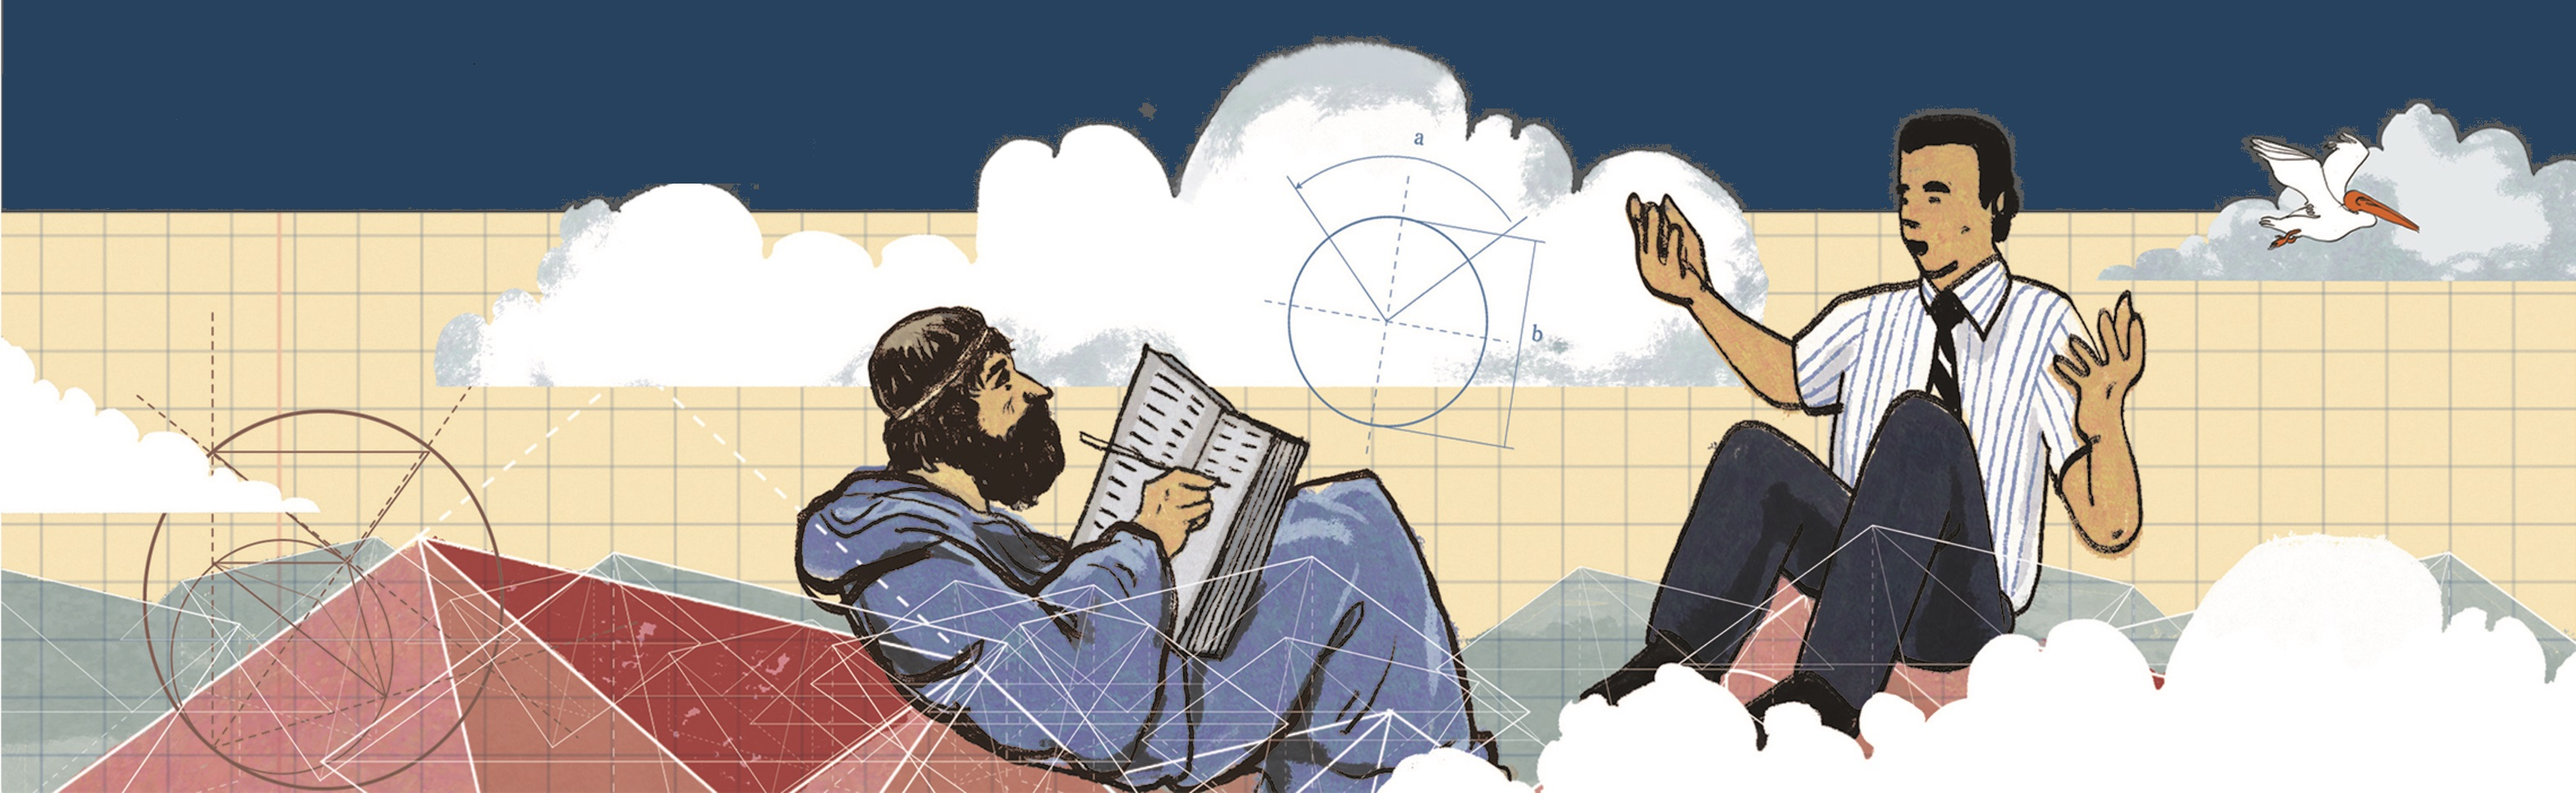
\includegraphics[width=19.3cm]{../bannerdoithoai}}}
\AddToShipoutPicture*{\put(50,500){
\includegraphics[scale=1]{../tieude.pdf}}}\centering
\endgroup

\vspace*{225pt}
\textit{\textbf{\color{doithoaitoanhoc}LTS.} Hélène Esnault ($1953$) là một nhà toán học đương đại nổi tiếng thế giới. Bà từng đọc báo cáo mời tiểu ban tại ICM $2002$, là Ủy viên Hội đồng xét giải thưởng Fields $2018$, Chủ tịch Hội đồng xét giải thưởng Shaw ($2021-2023$) và là thành viên của rất nhiều các ủy ban, hội đồng khác. Hélène Esnault cũng là một người bạn lâu năm thân thiết của các nhà toán học Việt Nam và là Tiến sỹ danh dự của Viện Hàn lâm Khoa học và Công nghệ Việt Nam. Tòa soạn trân trọng giới thiệu bài phỏng vấn Esnault do tờ báo Die Zeit (Thời báo), tuần báo lớn nhất của Đức, thực hiện. Trong bài phỏng vấn, Hélène Esnault chia sẻ về hành trình của mình, từ một đứa trẻ thông minh lớn lên trong gia đình lao động nghèo trở thành một giáo sư toán học, và những trải nghiệm trong nghiên cứu, ý nghĩa của toán học đối với con người và xã hội.}

\begin{multicols}{2}	
	Hélène Esnault lớn lên trong một gia đình lao động nghèo ở ngoại ô Paris, ngày nay bà là một trong những nhà toán học thành công nhất. Một cuộc trò chuyện về sự tò mò,\linebreak khoảnh khắc khai sáng trên đường cao tốc và nỗ lực của một cơ quan tình báo đề nghị bà cộng tác. Phỏng vấn của Stefan Klein.
	\vskip 0.1cm
	\textit{Hélène Esnault thuộc vào nhóm những nhà toán học thành công nhất trên thế giới, nhưng thay vì các công thức và tài liệu tham khảo về các chương trình nghiên cứu, trang web của bà có các bài thơ bằng tiếng Pháp, tiếng Anh, tiếng Đức và tiếng Nga. Một trong số đó là của \linebreak chính Esnault, nó nói là về sự gần gũi đã bị mất trong đại dịch. Esnault giải thích cho tôi, bà luôn viết, và ngày càng chuyển sang văn học nhiều hơn vì bà đang sống ở Đức và sợ quên dần tiếng tiếng Pháp mẹ đẻ.
		\vskip 0.1cm
		Sinh ra tại Paris năm $1953$, Esnault giữ vị trí Giáo sư mang tên Einstein tại Đại học Tự do Berlin trong một thời gian dài; nay bà đã nghỉ hưu. Bà mời tôi tới uống trà trong căn hộ của mình ở Schöneberg. Nhưng Esnault thích nói về thơ hơn. Trước đây vài giờ, một chứng minh có sự đóng góp của bà, mà các nhà toán học đã tìm kiếm trong gần bốn thập kỷ vừa được công bố trên mạng. Tiếng chuông liên tục từ máy tính xách tay của bà thông báo các email chúc mừng.}
	\vskip 0.1cm
	\textbf{\color{doithoaitoanhoc}Klein:} Esnault, điều gì đã đưa chị đến với toán học?
	\vskip 0.1cm
	\textbf{\color{doithoaitoanhoc}Hélène Esnault:} Thời con gái, tôi rất quan tâm đến ngôn ngữ, văn học và triết học. Tôi đọc rất nhiều. Nhưng ngay khi tôi mở miệng nói về những chủ đề này, mọi người đã nghe thấy tôi đến từ đâu. Tôi không thể thể hiện bản thân như mong đợi. Toán học thu hút tôi bởi vì nó không quan tâm bạn đến từ đâu. Đó là một phần của sự giải phóng của tôi.
	\vskip 0.1cm
	\textbf{\color{doithoaitoanhoc}Klein:} Chị đến từ đâu?
	\vskip 0.1cm
	\textbf{\color{doithoaitoanhoc}Esnault:} Từ một trong những vùng ngoại ô của Paris mà anh nhìn thấy trên TV khi tình\linebreak trạng bất ổn bạo lực thỉnh thoảng bùng lên. Lúc đầu, chúng tôi sống trong một căn phòng áp mái, không có nước máy. Tôi không có giường của riêng mình và bố mẹ tôi đã giao tôi cho một người khác nuôi vì không có đủ chỗ cho tôi. Tôi chỉ có thể quay lại gia đình mình vào lúc ba tuổi, khi chúng tôi được cấp một căn nhà ở xã hội. Cha tôi là một công nhân luyện kim. Ông rời trường học khi mới $12$ tuổi để kiếm sống. Tôi nói chuyện với ông bằng một thứ tiếng lóng của giới công nhân mà không một người Pháp lịch lãm nào thực sự hiểu được. Mẹ tôi là y tá trong nhà máy của cha tôi. Bà biết mông của hầu hết tất cả mọi người trong khu nhà của chúng tôi vì bà đã dùng những ống tiêm cũ để tiêm miễn phí cho bất kỳ ai cần.
	\vskip 0.1cm
	\textbf{\color{doithoaitoanhoc}Klein:} Trong môi trường đó, điều gì đã khiến chị theo đuổi con đường học thuật?  
	\vskip 0.1cm
	\textbf{\color{doithoaitoanhoc}Esnault:} Cha tôi rất hay đọc. Sau giờ làm việc, ông sẽ ôm những cuốn sách về lịch sử. Để hiểu ngữ pháp tiếng Pháp, ông đã tự học tiếng Tây Ban Nha, vì ngôn ngữ này có cấu trúc tương tự như ngôn ngữ của chúng tôi. Khi còn trẻ, ông đã tham gia các lớp học buổi tối, nơi những trí thức có lý tưởng dạy toán miễn phí cho công nhân. Khi còn là một thiếu niên, tôi cũng đã tham gia các khóa học này.
	\vskip 0.1cm
	\textbf{\color{doithoaitoanhoc}Klein:} Có ảnh hưởng của ông ấy lên quyết định của chị không?
	\vskip 0.1cm
	\textbf{\color{doithoaitoanhoc}Esnault:} Cũng có. Tôi đã nghe nói về vô hạn ở trường, điều này khiến tôi rất thích thú. Toán học dường như là một trò chơi bất tận đối với tôi. Trong cờ vua, thứ mà cha tôi rất giỏi, luôn có một người thắng và một người thua. Toán học ngược lại không bao giờ dừng. Câu hỏi mới nảy sinh từ mỗi câu trả lời. Và toán học đòi hỏi sự trung thực tuyệt đối. Gian lận là điều không thể chấp nhận được. Vì thế, tôi đã đi khắp Paris đến các khóa học dành cho công nhân. Tôi muốn biết thêm. Và tôi muốn xem làm thế nào để dạy toán cho những người, giống như cha tôi, có trình độ học vấn thấp.
	\begin{figure}[H]
		\centering
		\vspace*{-5pt}
		\captionsetup{labelformat= empty, justification=centering}
		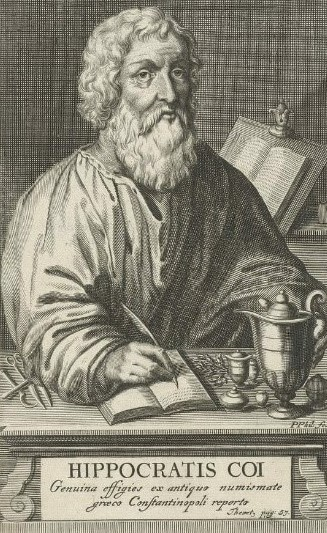
\includegraphics[width=0.65\linewidth]{1}
		\caption{\small\textit{\color{doithoaitoanhoc}Hélène Esnaut thời trẻ. (Ảnh từ bộ sưu tập của Viện Toán Oberwolfach).}}
		\vspace*{-10pt}
	\end{figure}
	\textbf{\color{doithoaitoanhoc}Klein:} Chị có trao đổi nhiều với cha mình về toán học không?
	\vskip 0.1cm
	\textbf{\color{doithoaitoanhoc}Esnault:} Không. Rất khó để nói chuyện với ông về toán. Ông đã nghe nói về số phức. Ông đã nhận ra một thực tế rằng những cấu trúc này của toán cao cấp dẫn đến những mối liên hệ không thể chứng minh được bằng những tính toán đơn giản. Tôi đã phải hứa sẽ giải thích tất cả những điều này cho ông một cách chi tiết.
	\vskip 0.1cm
	\textbf{\color{doithoaitoanhoc}Klein:} Ta không thể đếm bằng số phức vì chúng không được xếp trên một trục số mà trên một mặt phẳng. Số phức đơn giản nhất, được gọi là $i$, khi nhân với chính nó sẽ cho kết quả là $-1$. Thật khó để tưởng tượng.
	\vskip 0.1cm
	\textbf{\color{doithoaitoanhoc}Esnault:} Vâng, và tôi không đủ kiên nhẫn để giải thích điều đó với ông. Tôi đã rất sốt ruột và đang mắc kẹt trong hệ thống toán học. Phần lớn những gì cha tôi thắc mắc đã trở thành hiển nhiên với tôi. Tuổi trẻ thường\linebreak vô ơn.
	\vskip 0.1cm
	\textbf{\color{doithoaitoanhoc}Klein:} Có thầy cô nào đã hỗ trợ chị không?
	\vskip 0.1cm
	\textbf{\color{doithoaitoanhoc}Esnault:} Dạo đó thì không -- ngoại trừ việc cô hiệu trưởng trường tiểu học của tôi khuyên cha mẹ tôi nên gửi tôi đến trường trung học ở Paris. Sau đó, với ba franc mà tôi có, tôi mua cho mình những cuốn sách toán rách nát từ những người bán hàng bên bờ sông Seine, những người lúc đó không chỉ bán đồ lưu niệm cho khách du lịch mà còn bán cả sách, và thử sức với những bài tập trong đó. Sau khi tốt nghiệp trung học, bố mẹ tôi lại được gọi lên. Họ được cho biết rằng tôi nên tham gia một lớp học dự bị để thi vào một trong những trường đại học ưu tú có tên là Grande École, mà trong trường hợp của tôi là để học toán. Tôi thậm chí còn không có khái niệm rằng có thể học toán ở bậc đại học! Đối với tôi, hệ thống giáo dục thực sự hiệu quả.
	\vskip 0.1cm
	\textbf{\color{doithoaitoanhoc}Klein:} Các Grandes Écoles được coi là cực kỳ tư sản. Chị cảm thấy thế nào khi ở đó?
	\vskip 0.1cm
	\textbf{\color{doithoaitoanhoc}Esnault:} Cảm giác tò mò. Sau khi một bạn gái khác phải nghỉ học, tôi là nữ sinh duy nhất trong lớp dự bị. Trường trung học chuyên dành cho những lớp này thậm chí còn không có nhà vệ sinh riêng cho tôi. Nhưng có một chuyện khác quan trọng hơn nhiều. Sau vài tuần trong học kỳ đầu tiên, một cậu bé dường như thích tôi đã kéo tôi ra một chỗ. Có xì xào về tôi, cậu ấy kể. Thứ nhất là mọi người bàn tán chuyện tôi đến từ một khu phố nghèo. Thứ hai, cha tôi là một công nhân, và thứ ba, ông là cộng sản. Hai đầu gối tôi run lên. Bạn không nên lo lắng, cậu bạn trấn an tôi: tớ đã giải thích với những người khác rằng tất cả những điều này không thể đúng. Và tại sao? “Vì bạn luôn sạch sẽ và thơm tho.”
	\vskip 0.1cm
	\textbf{\color{doithoaitoanhoc}Klein:} Không thể tin được. Chị có nghĩ rằng mọi chuyện sẽ khác với mình nếu ở Đức?
	\vskip 0.1cm
	\textbf{\color{doithoaitoanhoc}Esnault:} Khi tôi còn làm việc tại Viện Toán học Max Planck ở Bonn, tôi là thành viên của một Ban tuyển chọn của Quỹ Học thuật Quốc gia Đức. Tôi phỏng vấn những ứng viên trong lĩnh vực của tôi. Có lần tôi có một ứng viên giải thích rất kỹ cho tôi về môn toán cao cấp mà anh ta đã tự học khi còn là một người lính nghĩa vụ nhàm chán. Sự hiểu biết của anh ấy thật ấn tượng. Anh là một đứa trẻ thuộc tầng lớp lao động và chưa bao giờ học. Ủy ban muốn từ chối anh ta vì anh ta thiếu hiểu biết về văn chương hay âm nhạc. Tôi đã phải thực hiện một cuộc đấu tranh để đủ phiếu ủng hộ anh ta. 
	\vskip 0.1cm
	\textbf{\color{doithoaitoanhoc}Klein:} Làm thế nào chị, một người bên lề, xoay sở để khẳng định mình?
	\vskip 0.1cm
	\textbf{\color{doithoaitoanhoc}Esnault:} Cha tôi đã dạy tôi tính kiên trì. Bản thân ông rất thể thao và điều đó đã sống cứu ông. Nếu không thì ông đã không sống sót sau cú nhảy khỏi đoàn tàu hỏa hướng tới Buchenwald. Đức Quốc xã muốn đưa ông vào trại tập trung vì là người cộng sản kháng chiến. Nhưng khi đoàn tàu lăn bánh qua miền Bắc nước Pháp, ông và khoảng mười đồng đội đã thoát khỏi những loạt đạn của quân Đức. Những người cuối cùng bị trúng đạn, cha tôi chạy nhanh hơn họ. Lúc đó ông đã ngoài ba mươi và có lúc còn kéo theo một đồng đội bị thương. Ông không bao giờ kể thêm về giai đoạn đó. Khi tôi còn là một đứa trẻ, ông nói rất nhiều về đạp xe, một môn thể thao của tầng lớp lao động vào thời điểm đó. Ông tuyên bố rằng các cuộc đua như Tour de France khắc nghiệt đến nỗi chỉ có những người lao động mới vượt qua nổi: ``Chỉ chúng ta mới có thể chịu đựng được.” Tôi không muốn trở thành vận động viên. Nhưng ông đã đúng: Ai sinh ra không có đặc ân, sẽ bù đắp thiệt thòi bằng ý chí kiên cường.
	\vskip 0.1cm
	\textbf{\color{doithoaitoanhoc}Klein:} Và những ý chí như vậy cần thiết trong toán học?
	\vskip 0.1cm
	\textbf{\color{doithoaitoanhoc}Esnault:} Ồ vâng. Công việc của chúng tôi rất căng thẳng. Có những giai đoạn bạn giải quyết một vấn đề cả ngày lẫn đêm. Khi sinh viên muốn làm nghiên cứu sinh với tôi, điều đầu tiên tôi hỏi họ là: Bạn có thể sống với điều gì đó thường xuyên ám ảnh bạn không? 
	\vskip 0.1cm
	\textbf{\color{doithoaitoanhoc}Klein:} Giống như một con ma?
	\vskip 0.1cm
	\textbf{\color{doithoaitoanhoc}Esnault:} Vâng. Các bạn trẻ phải chịu đựng được điều đó. Bạn cần tình yêu với toán học, cũng như sự sẵn sàng hy sinh. Nếu không thì đó là một sự tồn tại khốn khổ. Bởi vì toán học mạnh hơn chúng tôi, bạn thấy mình trong một trận chiến liên tục. Tôi không thích từ chiến đấu, nhưng tôi không biết cách diễn đạt nào khác tốt hơn: Bạn muốn hiểu nhưng bạn không thể. Ví dụ, tôi đã có một vấn đề trong đầu trong hai năm mà tôi không thể giải quyết được. Và mỗi khi tôi cố gạt nó sang một bên, nó lại quay trở lại. Tôi biết chắc rằng đó là một vấn đề khá nhỏ. Nhưng khi cuối cùng tôi đã giải quyết được nó, có lẽ nó sẽ giúp người ta hiểu được một vài mối liên hệ khác.
	\vskip 0.1cm
	\textbf{\color{doithoaitoanhoc}Klein:} Chính xác thì chị đang nghiên cứu gì?
	\vskip 0.1cm
	\textbf{\color{doithoaitoanhoc}Esnault:} Hình học đại số số học. Chúng tôi nghiên cứu lý thuyết số với sự trợ giúp của các hình ảnh hình học.
	\vskip 0.1cm
	\textbf{\color{doithoaitoanhoc}Klein:} Nếu tôi hiểu đúng, một câu hỏi đơn giản, chẳng hạn là, những phân số nào là nghiệm một phương trình như $x^2 + y^2 = 1$ -- và chúng có tồn tại hay không. Phương \linebreak trình này xác định một đường tròn có bán kính bằng $1$.
	\begin{figure}[H]
		\centering
		\vspace*{-5pt}
		\captionsetup{labelformat= empty, justification=centering}
		
\includegraphics[width=0.65\linewidth]{2}
		%		\caption{\small\textit{\color{doithoaitoanhoc}Hélène Esnaut thời trẻ. (Ảnh từ bộ sưu tập của Viện Toán Oberwolfach).}}
		\vspace*{-10pt}
	\end{figure}
	\textbf{\color{doithoaitoanhoc}Esnault:} Chính xác, chúng tôi nghiên cứu các đa tạp đại số trên các trường khác nhau. Một điều tuyệt vời mới xảy ra: Một nhóm các nhà toán học gồm một người Úc, một người Ấn Độ và một người Canada đã thành công trong việc chứng minh dạng tổng quát nhất của một giả thuyết đã tồn tại trong hơn $35$ năm về sự phân bố các điểm đặc biệt trên các đa tạp Shimura\footnote{\color{doithoaitoanhoc}Xem bài “Một chứng minh cho giả thuyết $30$ năm của André và Oort” trong Pi số này.”}. Chứng minh, vừa được công bố sáng nay, và bây giờ phải được các chuyên gia kiểm tra, có sử dụng một kết quả căn bản mà một nhà toán học trẻ tuổi và tôi đã phát hiện ra. 
	\vskip 0.1cm
	\textbf{\color{doithoaitoanhoc}Klein:} Tôi cũng xin chúc mừng! Tuy nhiên, tôi sợ rằng bây giờ với tôi cũng giống như với cha của chị: Thật không may, tôi không hiểu ý nghĩa các kết quả này. Dù giống như mọi nhà vật lý khác, tôi đã hoàn thành chương \linebreak trình đại học về toán học. Có bao nhiêu người trên thế giới thực sự hiểu chị đang làm gì?
	\vskip 0.1cm
	\textbf{\color{doithoaitoanhoc}Esnault:} Điều đó phụ thuộc vào ý của anh khi nói “hiểu”. Tôi không biết liệu tôi có nên tiết lộ bao nhiêu người có thể hiểu chi tiết công việc của chúng tôi. Câu trả lời có thể không làm hài lòng các nhà tài trợ ở các quỹ nghiên cứu quốc gia.
	\vskip 0.1cm
	\textbf{\color{doithoaitoanhoc}Klein:} Để tôi đoán: đếm trên đầu ngón tay?
	\vskip 0.1cm
	\textbf{\color{doithoaitoanhoc}Esnault:} Đôi khi chỉ có ba. Nhưng hình học đại số số học nói chung là một lĩnh vực lớn. Trong lĩnh vực này, nếu tính rất hào phóng, có khoảng vài trăm nhà toán học trên khắp thế giới.
	\vskip 0.1cm
	\textbf{\color{doithoaitoanhoc}Klein:} Nói về các nhà tài trợ: Phần còn lại của thế giới hưởng lợi như thế nào từ những phát hiện của anh chị?
	\vskip 0.1cm
	\textbf{\color{doithoaitoanhoc}Esnault:} Không phải ngay lập tức. Toán học có động lực riêng của nó. Các vấn đề đến với chúng tôi từ các ngành khoa học khác. Ban đầu, các nhà vật lý, nhà khoa học máy tính hoặc nhà sinh học quan tâm đến cách một cái gì đó có thể được tính toán. Các nhà toán học suy nghĩ và tiếp tục xoay vòng các ý tưởng của họ. Sau mấy năm, những suy nghĩ trở nên trừu tượng đến mức người ta thường không thể hiểu được vấn đề ban đầu xuất phát \linebreak từ đâu.
	\vskip 0.1cm
	\textbf{\color{doithoaitoanhoc}Klein:} Khi đó toán học sẽ giống như một trò ghép hình mà các anh chị đặt ra theo ý thích của riêng mình.
	\vskip 0.1cm
	\textbf{\color{doithoaitoanhoc}Esnault:} Đúng, nhưng một trò ghép hình không chỉ trải trên mặt bàn, mà còn ở nhiều chiều khác. Đôi khi, một cái nhìn sâu sắc từ trò chơi cho thấy công dụng thực tế đáng ngạc nhiên trong nhiều thập kỷ sau đó. Nhưng thường thì không. Tôi luôn biết rằng tôi muốn làm những việc xa rời tất cả các ứng dụng. Toán học càng thuần túy càng tốt. Khi còn là một nhà toán học trẻ, tôi thường sợ rằng giới quân sự sẽ lạm dụng công việc của tôi. Việc các công thức đã được sử dụng để chế tạo bom nguyên tử đã rất ảnh hưởng tới tôi.
	\vskip 0.1cm
	\textbf{\color{doithoaitoanhoc}Klein:} Tại sao lại nên dành cả cuộc đời\linebreak mình cho những bài toán mà hầu như không ai hiểu? Và rất không chắc chắn liệu các lời giải có mang lại lợi ích cho ai hay không?
	\vskip 0.1cm
	\textbf{\color{doithoaitoanhoc}Esnault:} Đó chưa bao giờ là một câu hỏi đối với tôi. Chúng ta làm rất nhiều điều vô ích và sống tốt với chúng. Trong mắt tôi, sức hấp dẫn của toán học chính là nằm ở tính trừu tượng.
	\vskip 0.1cm
	\textbf{\color{doithoaitoanhoc}Klein:} Nhiều người lạ lẫm với sự trừu tượng -- đối với họ, các ký hiệu toán học, biểu diễn những thứ không chạm tới được, là trống rỗng về nội dung. Tôi đoán, đó là lý do thực sự tại sao nhiều người đã gặp rắc rối với toán học ngay từ thời học phổ thông.  
	\vskip 0.1cm
	\textbf{\color{doithoaitoanhoc}Esnault:} Các nhà toán học chúng tôi chỉ đơn giản là cố gắng lược bỏ nhiều nhất những rườm rà trong suy nghĩ của mình, để phát biểu mọi thứ ngắn gọn và tổng quát nhất có thể. Hoạt động của chúng tôi tương tự như hoạt động của một nhà thơ đấu tranh cho ngôn ngữ của mình. Chúng tôi thử các công thức, thêm một câu ở đây, lấy thứ gì ở đó. Và nếu mọi thứ suôn sẻ, đến một lúc nào đó bạn có cảm giác rằng nó đúng. Nhưng ngoài những yếu tố tạo ra mỗi liên hệ giữa toán học và nghệ thuật, giữa chúng vẫn có một khác biệt lớn: Nghệ thuật cho phép nhiều câu trả lời. Chúng tôi có một tiêu chí về chân lý. Chỉ có đúng và sai.
	\vskip 0.1cm
	\textbf{\color{doithoaitoanhoc}Klein:} Chị hiểu Chân lý như thế nào?
	\vskip 0.1cm
	\textbf{\color{doithoaitoanhoc}Esnault:} Theo cách hiểu thông thường thì đó Sự thật. Trong Toán học chúng tôi hiểu đó là sự đúng đắn. Nghĩa là không có sự mâu thuẫn giữa các khẳng định. Mỗi mệnh đề được viết ra phải phù hợp với hàng triệu \linebreak mệnh đề khác. Đó là một yêu cầu rất cao: với mỗi khẳng định cần có một chứng minh,\linebreak rằng nó không đưa đến bất kỳ mâu thuẫn nào. Như thế, Toán học là một lâu đài Chân lý.
	\vskip 0.1cm
	\textbf{\color{doithoaitoanhoc}Klein:} Thế lâu đài của những suy nghĩ chân lý này từ đâu ra? Nhiều nhà toán học và một số triết gia nói rằng nó luôn ở đó. Mọi người chỉ có nhiệm vụ khám phá nó. Galileo gọi toán học là ``bảng chữ cái mà Chúa dùng để mô tả vũ trụ".
	\vskip 0.1cm
	\textbf{\color{doithoaitoanhoc}Esnault:} Tôi nghĩ rằng lâu đài này do con người chúng ta xây dựng. Chúng tôi tò mò và phát minh ra các công cụ trí tuệ mới để hiểu. Những câu hỏi mới nảy sinh từ những công cụ này, v.v. Do đó, trong hàng nghìn năm kể từ khi người Sumer và người Trung Quốc đặt nền móng đầu tiên, toán học đã phát triển.
	\vskip 0.1cm
	\textbf{\color{doithoaitoanhoc}Klein:} Vậy thì chị phải giải thích tại sao toán học lại tiên đoán rất nhiều hiện tượng mà con người chưa bao giờ quan sát được. Hãy nghĩ về lý thuyết tương đối. Chỉ với các công thức của toán học, Einstein và các nhà vật lý khác đã có thể dự đoán lỗ đen hơn một trăm năm trước. Chúng ta đã nhìn thấy hình ảnh đầu tiên về một lỗ đen vào năm $2019$.
	\vskip 0.1cm
	\textbf{\color{doithoaitoanhoc}Esnault:} Đối với tôi, những thành công như vậy cho thấy chúng tôi đã làm rất tốt. Nếu một công cụ có thể được sử dụng cho những mục đích mà người tạo ra nó chưa bao giờ nghĩ đến, thì thật là tốt. Tôi đã tự trải nghiệm ví dụ khác. NSA Hoa Kỳ đã hai lần cố gắng mời tôi tôi làm phản biện.
	\vskip 0.1cm
	\textbf{\color{doithoaitoanhoc}Klein:} Cơ quan tình báo đã suy sụp sau tiết lộ của Edward Snowden?
	\vskip 0.1cm
	\textbf{\color{doithoaitoanhoc}Esnault:} Vâng. Họ đã phát hiện ra rằng các quá trình mã hóa các thông điệp bí mật có thể được rút ra từ kiến thức về hình học đại số. Tôi đã từ chối cả hai lần.
	\vskip 0.1cm
	\textbf{\color{doithoaitoanhoc}Klein:} Mặc dù vậy, chị đã không thực sự \linebreak thành công trong cố gắng không làm bất cứ điều gì hữu ích để tránh giới quân sự trong mọi trường hợp.
	\vskip 0.1cm
	\textbf{\color{doithoaitoanhoc}Esnault:} Giới quân sự không quan tâm trực tiếp đến kết quả nghiên cứu của tôi. Nhưng vâng, tôi đã rất ngây thơ. Toán học không chỉ là về nội dung, nó kiểm tra chính những lập luận logic. Nhưng đó chính là lý do khiến nó không vô dụng. Tại sao nền kinh tế Đức thuê các nhà toán học?
	\vskip 0.1cm
	\textbf{\color{doithoaitoanhoc}Klein:} Họ thiết kế phần mềm hoặc quản lý rủi ro.
	\vskip 0.1cm
	\textbf{\color{doithoaitoanhoc}Esnault:} Họ chưa bao giờ được học về các quy trình trong một công ty trong quá trình\linebreak đào tạo của mình. Thay vào đó họ được học cách bỏ qua các chi tiết và nhận ra cấu trúc đằng sau của vấn đề. Có thể nói họ có một con mắt tinh tường nhìn thấy cái gì phụ thuộc cái gì và làm thế nào để sắp xếp mọi thứ theo trật tự tốt nhất.
	\vskip 0.1cm
	\textbf{\color{doithoaitoanhoc}Klein:} Chị làm thế nào để tiếp cận một vấn đề phức tạp? Chẳng hạn, chị có thử hình dung các mối quan hệ bằng hình ảnh hoặc trên giấy không?
	\vskip 0.1cm
	\textbf{\color{doithoaitoanhoc}Esnault:} Khó nói. Anh có biết mình mơ bằng ngôn ngữ nào không?
	\vskip 0.1cm
	\textbf{\color{doithoaitoanhoc}Klein:} Thường bằng tiếng Đức. Sau một vài tuần ở một đất nước mà ngôn ngữ tôi có thể nói, điều đó sẽ thay đổi. Chị có trải qua những suy nghĩ căng thẳng như một trạng thái mơ không?
	\vskip 0.1cm
	\textbf{\color{doithoaitoanhoc}Esnault:} Chừng nào tôi còn chưa hiểu vấn đề, tôi cảm thấy như mình đang ở trong màn sương dày đặc. Sau đó, tôi hầu như không nhận thấy những gì đang xảy ra trong tôi và với tôi. Tôi thường viết hoặc nguệch ngoạc những bức vẽ nhỏ, một mặt để xua đi tâm lý hồi hộp, mặt khác đó là cách tiếp cận vấn đề. Nhưng có những nhà toán học không cần tay để suy nghĩ. Họ thậm chí không ghi chú. Với họ, mọi thứ diễn ra trong đầu.
	\vskip 0.1cm
	\textbf{\color{doithoaitoanhoc}Klein:} Albert Einstein đã từng viết rằng ý tưởng của ông phát triển trong các hình ảnh nội tại, nhưng cũng trong ``những suy nghĩ sơ đẳng”, mà ông cho là tác nhân cơ bắp. Rõ ràng là ông ta suy nghĩ với cả cơ thể. Mặt khác, ngôn ngữ với tư cách là một công cụ của tri thức, hầu như không đóng một vai trò nào đối với ông.
	\vskip 0.1cm
	\textbf{\color{doithoaitoanhoc}Esnault:} Tôi không thể xác nhận điều đó đối với bản thân mình. Một ý nghĩ chỉ thực sự rõ ràng với tôi khi tôi có thể viết nó ra một cách gọn gàng. Tôi cũng tự hỏi ngôn ngữ ảnh hưởng đến tư duy logic của chúng ta như thế nào. Ví dụ trong tiếng Nhật, bạn không nói “không” vì điều đó được coi là bất lịch sự. Mặt khác, tiếng Đức dường như đặc biệt phù hợp với logic và toán học.
	\vskip 0.1cm
	\textbf{\color{doithoaitoanhoc}Klein:} Tại sao?
	\vskip 0.1cm
	\textbf{\color{doithoaitoanhoc}Esnault:} Bởi vì ngữ pháp tiếng Đức tạo ra khả năng diễn đạt các mức độ khác nhau của sự thật. Khi người Đức diễn đạt tình huống ``Anh ta nói, anh ta đã cư xử như vậy”, họ thể hiện tính khách quan của lời nói bằng cách sử dụng các động từ ``nói” và ``cư xử” ở hai thể khác nhau. Tất cả các ngôn ngữ khác mà tôi biết đều không phân biệt được thực tế và nội dung của khẳng định, chúng sử dụng các động từ ``nói” và ``cư xử” trong tình huống trên ở cùng một thể. Tôi luôn thấy độ chính xác này là một thế mạnh lớn. Ngôn ngữ Đức đã làm phong phú thêm cho tôi rất nhiều. Nhưng có lẽ việc một người đi đến cái nhìn sâu sắc thông qua ngôn ngữ, hình ảnh hoặc cảm giác cơ thể không phải là quan trọng -- trong mọi trường hợp, có những khoảnh khắc hạnh phúc lúc chúng ta có cảm giác rằng chúng ta hiểu được điều gì đó.
	\vskip 0.1cm
	\textbf{\color{doithoaitoanhoc}Klein:} Chị trải qua những khoảnh khắc này như thế nào?
	\vskip 0.1cm
	\textbf{\color{doithoaitoanhoc}Esnault:} Chúng gần như luôn gây bất ngờ. Sau khi đứng trong bóng tối nhiều tuần hoặc thậm chí nhiều năm, đột nhiên bạn bước ra ánh sáng. Một lần, một liên hệ quan trọng mà tôi đã tìm kiếm bấy lâu bỗng nhiên hiện ra khi tôi đang lái xe trên một con đường cao tốc tại Bỉ. Thông thường tôi khá bình tĩnh. Nhưng lần đó hình ảnh gần như trọn vẹn, và tôi suýt hét lên. Thêm hai tuần nữa tôi mới viết được chứng minh ra giấy.
	\begin{figure}[H]
		\centering
		\vspace*{-5pt}
		\captionsetup{labelformat= empty, justification=centering}
		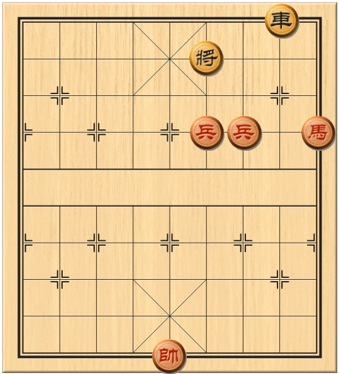
\includegraphics[width=1\linewidth]{3}
		\caption{\small\textit{\color{doithoaitoanhoc}Hélène Esnault cùng với Moritz Kerz (trái) và Alexander Beilinson (phải). (Ảnh từ trang web của Hélène Esnault).}}
		\vspace*{-10pt}
	\end{figure}
	\textbf{\color{doithoaitoanhoc}Klein:} Tôi thấy thú vị là tại khoảnh khắc khai sáng, chị đã nhận ra lời giải, nhưng vẫn chưa thể diễn đạt nó. Như thể có một kiến thức chưa thể diễn ngôn. Nhiều người gọi đây là trực giác.
	\vskip 0.1cm
	\textbf{\color{doithoaitoanhoc}Esnault:} Tôi gọi đó là niềm tin có cơ sở. Trong một thời gian ngắn, tôi đã luyện tập môn leo núi trong nhà. Đôi khi bạn phải vượt qua một cái vực với một bước nhảy xa và dứt khoát. Tôi thường bị chóng mặt trong tình huống này và khi đó các bạn tập thuyết phục tôi: Cứ nhảy đi nào! Bạn gần như đã ở phía bên kia, bạn có thể làm được. Đó là cảm giác của tôi khi ý tưởng đúng đắn đột nhiên nảy \linebreak sinh sau một thời gian dài nghi ngờ. Tất nhiên, câu hỏi đặt ra là: sự chắc chắn đạt được này đến từ đâu?
	\vskip 0.1cm
	\textbf{\color{doithoaitoanhoc}Klein:} Những người bạn tập của chị biết rằng chị sẽ làm được điều đó vì họ đã từng nhìn thấy nhiều người leo núi trước vực. Tôi đoán rằng rằng nếu chúng ta đã thực hiện một hoạt động trong nhiều năm, chúng ta sẽ sở hữu, một cách vô thức, một khối lượng lớn những kiến thức thực nghiệm. Chúng ta sẽ cảm nhận được điều gì khả thi khi gặp lại một tình huống đã biết, nhưng không thể mô tả điều đó.
	\vskip 0.1cm
	\textbf{\color{doithoaitoanhoc}Esnault:} Vâng, đúng là như vậy. Trước khi lời giải đến với tôi trên đường cao tốc Bỉ, tôi đã đọc rất nhiều về bản chất toán học của vấn đề đó. Vì thế, logic của nó đã trở nên quen thuộc với tôi đến mức tôi có thể nhìn rõ định hướng chính, ngay cả khi tôi vẫn còn thiếu nhiều chi tiết.
	\vskip 0.1cm
	\textbf{\color{doithoaitoanhoc}Klein:} Thật ngạc nhiên, chính các nhà toán học, không phải nhà tâm lý học hay nghệ sĩ, là những người đầu tiên nghiêm túc khám phá tư duy sáng tạo trong thế kỷ trước. Tôi nghĩ họ day dứt hơn ai hết về việc khoa học của họ dựa nhiều vào các quá trình vô thức. Ngày nay, một số chuyên gia khẳng định rằng trong năm mươi năm nữa máy tính sẽ trở \linebreak thành nhà toán học giỏi hơn. Chị có nghĩ vậy không?
	\vskip 0.1cm
	\textbf{\color{doithoaitoanhoc}Esnault:} Hãy nghĩ về Peter Scholze.
	\vskip 0.1cm
	\textbf{\color{doithoaitoanhoc}Klein:} Giám đốc Viện Toán học Max Planck ở Bonn, năm $2018$ là người Đức thứ hai nhận được Huy chương Fields, huy chương danh giá nhất cho các nhà toán học. Chị đã ở trong hội đồng xét.
	\vskip 0.1cm
	\textbf{\color{doithoaitoanhoc}Esnault:} Vâng. Nhưng Scholze đạt được \linebreak vinh quang không nhờ vào tôi, mà nhờ \linebreak thành tựu toán học tuyệt vời của anh ấy. Tôi chỉ làm nhiệm vụ của mình. Tháng Mười hai năm ngoái, anh ấy đã công bố một chứng \linebreak minh quan trọng, kết nối các lĩnh vực toán học khác nhau lại với nhau. Nhưng vì các lập luận mới lạ và rất phức tạp, Scholze không chắc chắn về chứng minh của mình và tìm sự giúp đỡ. Các nhà toán học đã đưa chứng \linebreak minh vào máy tính, mất nửa năm. Máy tính đã xác nhận cho Scholze.
	\vskip 0.1cm
	\textbf{\color{doithoaitoanhoc}Klein:} Nhưng máy tính chỉ kiểm tra chứng minh. Liệu nó có thể đưa ra một chứng minh không?
	\vskip 0.1cm
	\textbf{\color{doithoaitoanhoc}Esnault:} Chính xác. Máy tính chỉ phản hồi. Và nó chỉ nói ngôn ngữ mà chúng tôi đã dạy. Ngược lại, tư duy con người có thể bứt lên.
	\vskip 0.1cm
	\textbf{\color{doithoaitoanhoc}Klein:} Câu hỏi đặt ra là tại sao con người chúng ta lại có thể đạt đến tầm cao trí tuệ của toán học. Đối với tổ tiên thảo nguyên của chúng ta, việc sở hữu một bộ não hiểu được hình học đại số không mang lại lợi thế sinh tồn nào.
	\vskip 0.1cm
	\textbf{\color{doithoaitoanhoc}Esnault:} Đúng, nhưng mọi sự trừu tượng đều làm cho cuộc sống dễ dàng hơn vì nó rút ngắn đường đi của suy nghĩ. Nó bắt đầu với việc đếm một, hai, ba dễ dàng hơn so với việc đặt tên chi tiết cho tất cả các đối tượng mỗi lần. Thay vào đó, chúng ta nhóm mọi thứ lại với nhau dựa trên một số đặc điểm nhất định. Toán học là nghệ thuật đơn giản hóa.
	\begin{figure}[H]
		\centering
		\vspace*{-5pt}
		\captionsetup{labelformat= empty, justification=centering}
		
\includegraphics[width=1\linewidth]{4}
		\caption{\small\textit{\color{doithoaitoanhoc}Hélène Esnault và các đồng nghiệp trong Hội thảo về Đại số giao hoán và Hình học Đại số, Hà Nội, $1996$. (Ảnh từ bộ sưu tập của Viện Toán học).}}
		\vspace*{-10pt}
	\end{figure}
	\textbf{\color{doithoaitoanhoc}Klein:} Nhà toán học và nhà nghiên cứu não bộ Stanislas Dehaene từ Paris lập luận rằng chúng ta có cảm nhận về các con số. Tâm trí của chúng ta được lập trình để đếm mọi thứ. Trên thực tế, các thí nghiệm mới cho thấy trẻ sơ sinh có thể đếm mọi thứ chúng nhìn thấy và nghe thấy chỉ vài giờ sau khi sinh. Nhưng nếu mọi người được sinh ra với tài năng toán học, tại sao rất ít người có thể sử dụng nó?
	\vskip 0.1cm
	\textbf{\color{doithoaitoanhoc}Esnault:} Vì sự phát triển của các kỹ năng còn phụ thuộc vào sự giáo dục và xã hội. Đó là lý do tôi hài lòng về sự phổ biến của máy \linebreak tính. Chúng thách thức nhiều người suy nghĩ trừu tượng hơn bao giờ hết -- ngay cả những người lẽ ra không bao giờ tiếp xúc với toán học. Ngay những tin tặc cũng thường không có xuất thân xuất sắc. Nhưng khi tự học lập trình, họ có thể trở nên vô cùng sáng tạo. Tôi ước chúng ta có thể cho những người trẻ này nhiều cơ hội hơn để sử dụng tốt sự khéo léo của họ. Tôi đã phải để một trong những nhân viên giỏi nhất của mình tại Đại học Tự do Berlin ra đi sau khi vị trí của anh ta hết hạn. Tôi đã làm mất anh ta cho một cơ quan tình báo. Với tư cách là cấp trên của anh ấy, tôi đã được phỏng vấn để kiểm tra an ninh về anh ấy. Điều đó khiến trái tim tôi rỉ máu.
	\vskip 0.1cm
	\textbf{\color{doithoaitoanhoc}Klein:} Chị sẽ chọn nghề gì nếu không phát hiện ra toán học khi còn trẻ?
	\vskip 0.1cm
	\textbf{\color{doithoaitoanhoc}Esnault:} Có lẽ tôi đã vào tù. Khi mới lớn, tôi có rất nhiều uất ức trước sự bất công của thế giới khiến tôi có thể đã hủy hoại mọi thứ. Và khả năng làm một điều gì đó với kết thúc tồi tệ trong hoàn cảnh của tôi là không hề nhỏ. Cũng có thể tôi theo con đường viết văn.
	\vskip 0.1cm
	\begin{tBox}
		Stefan Klein, $55$ tuổi, nghiên cứu vật lý và triết học. Tại Klein, ông tổ chức các buổi nói chuyện về các chủ đề khoa học. Gần đây, cuốn sách ``Sáu tỉ đường đến hạnh phúc” của ông đã được dịch sang tiếng Việt (NXB Thế Giới). Một cuốn sách khác của ông, nhan đề ``Wir alle sind Sternenstaub” (Chúng ta đều là bụi từ các ngôi sao) sẽ tiếp tục được giới thiệu với bạn đọc Việt Nam trong thời gian tới. 
		\begin{figure}[H]
			\centering
			\vspace*{-5pt}
			\captionsetup{labelformat= empty, justification=centering}
			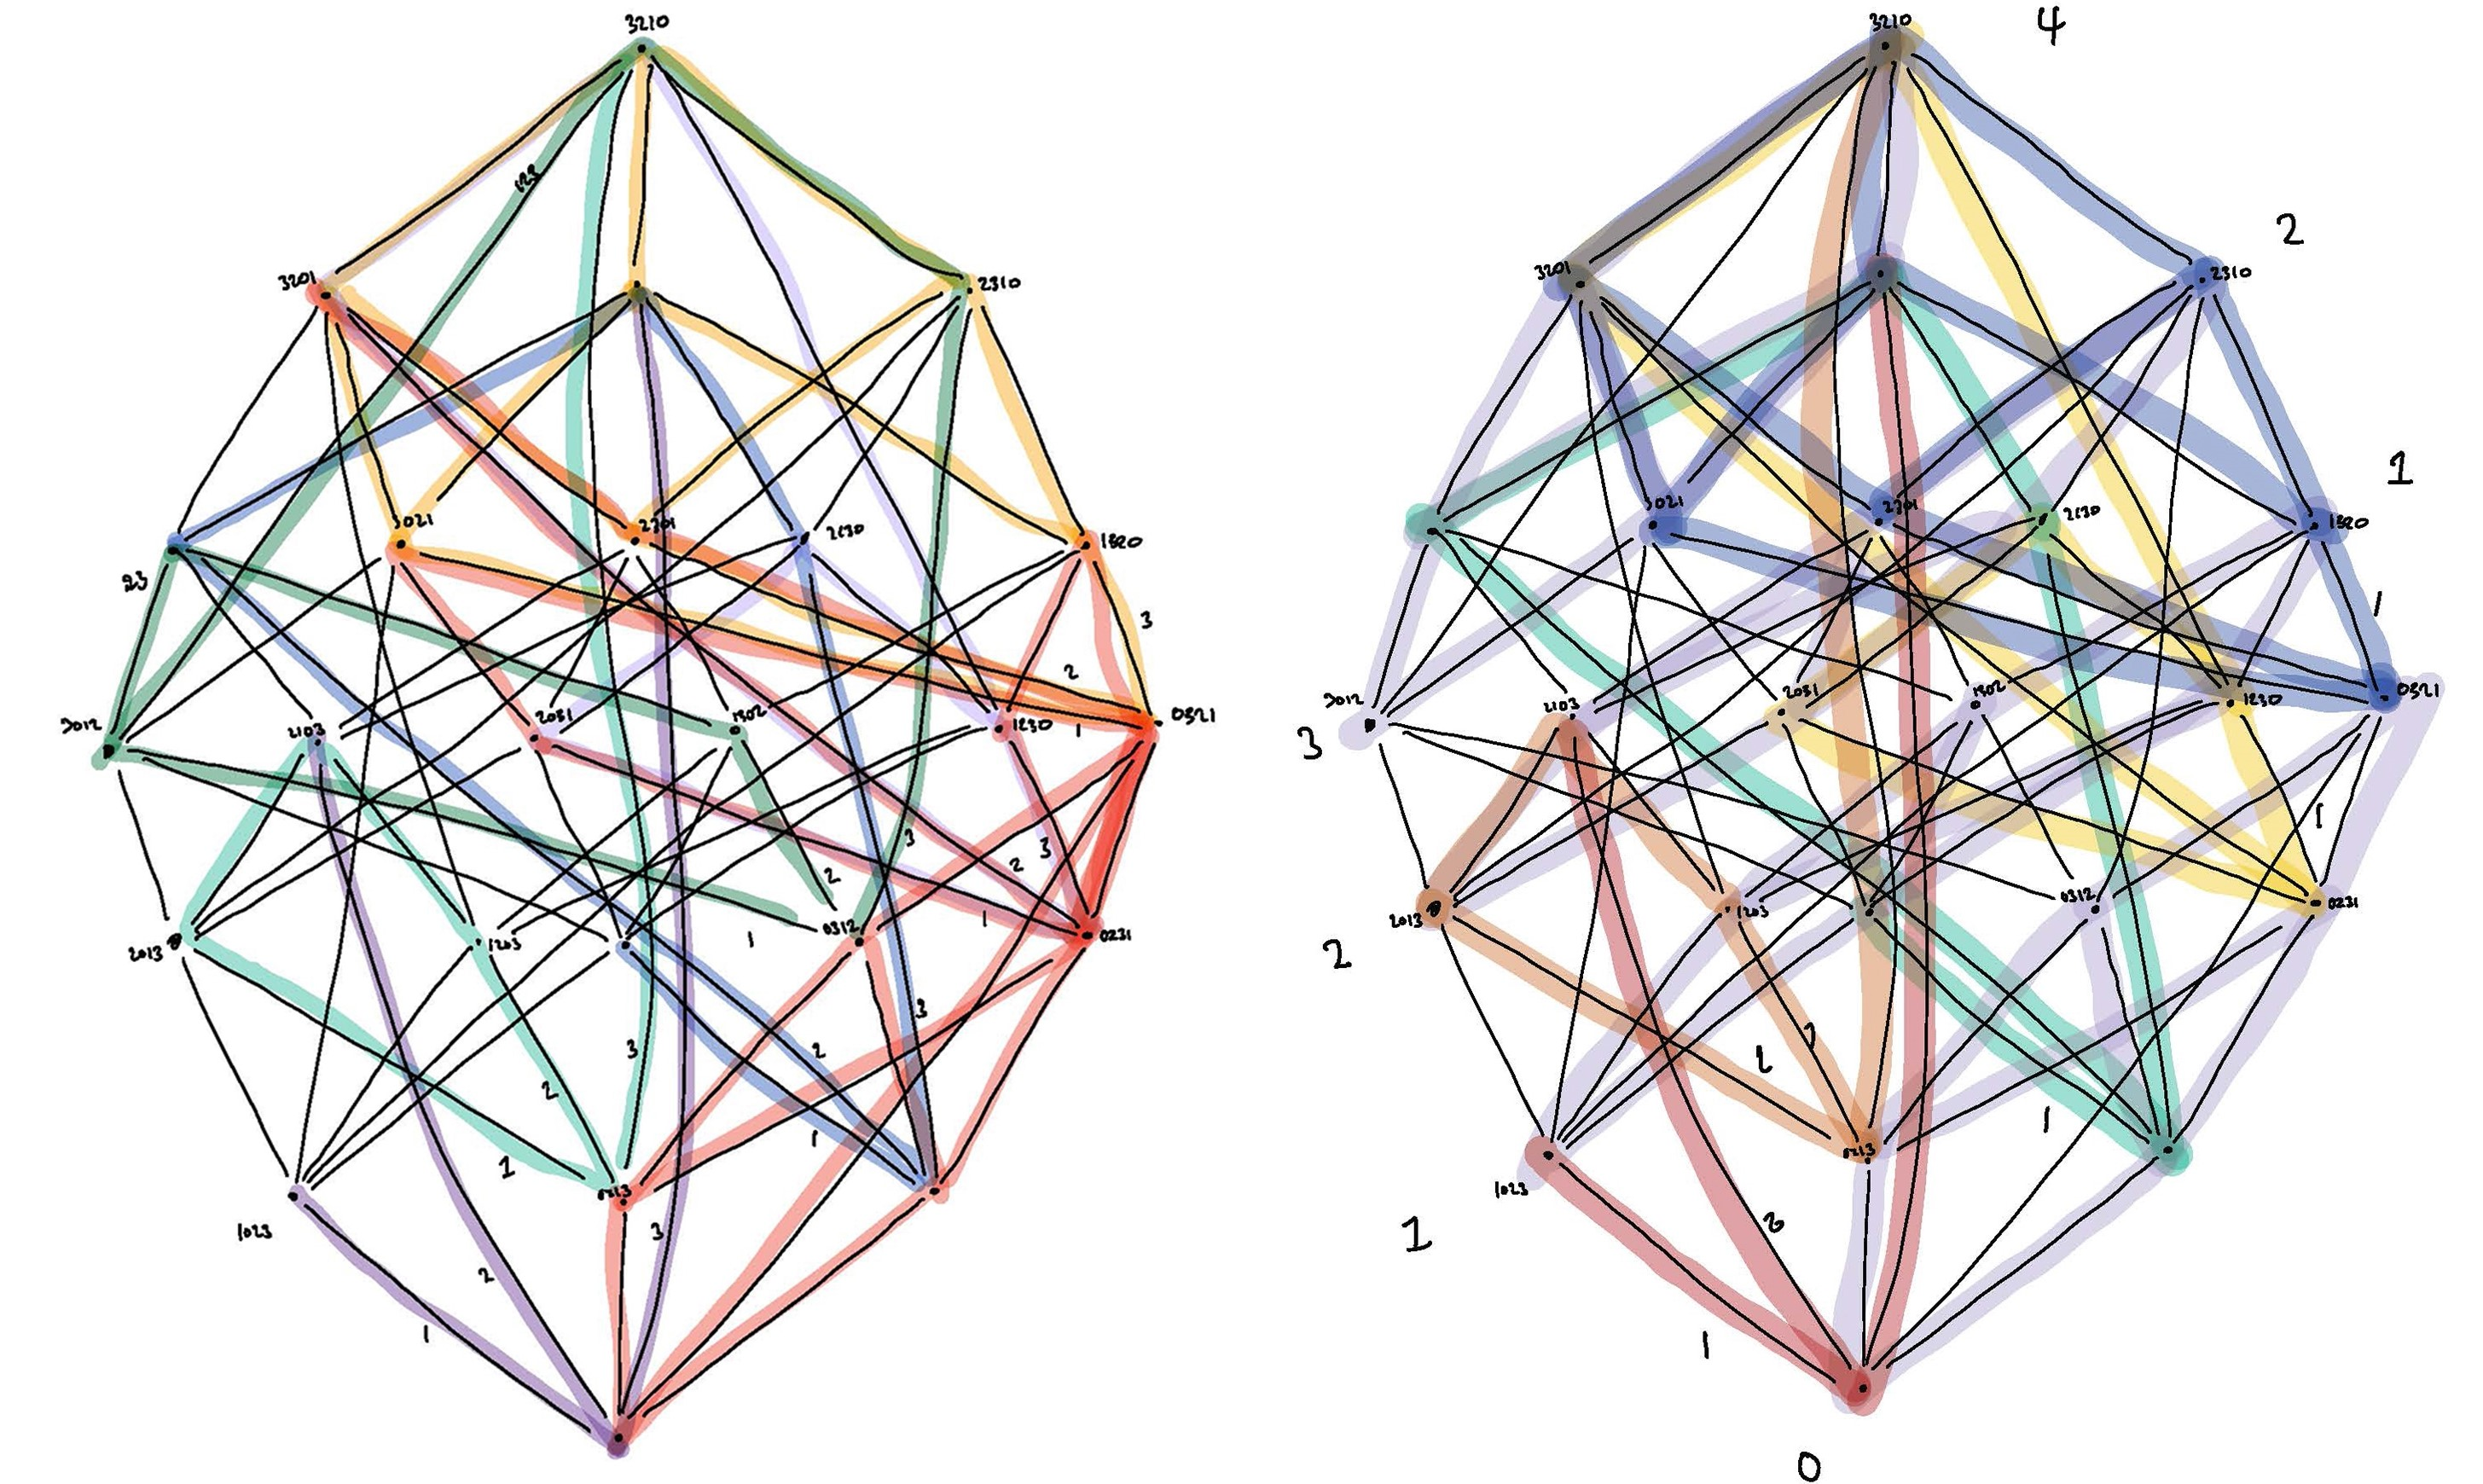
\includegraphics[width=0.55\linewidth]{5}
			%		\vspace*{-5pt}
		\end{figure}
	\end{tBox}
\end{multicols}
